\chapter{System Description}\label{chap:systemDescribtion}
The overall idea of the project is to consider more than one satellites flying in formation, with a certain distance in between and with the purpose of maintaining that distance by using the drag force. As a proof of concept, an AAU-CubeSat will be used, by choosing six AAU-CubeSat that orbit the Earth like is shown in  \figref{fig:1}. Therefore, a control system is developed, where the six satellites are nodes and they represent periods. Each satellite can only communicat with his two neighbour. In this project, all CubeSat's will be assumed identical, where each satellite needs to fulfill a few requirements stated in \chapref{chap:requirements}. Moreover, a full-scale implementation of the system will not be possible, therefore, the whole system will be simulated using MATLAB and Simulink. 
%
\begin{figure}[H]
	\centering
	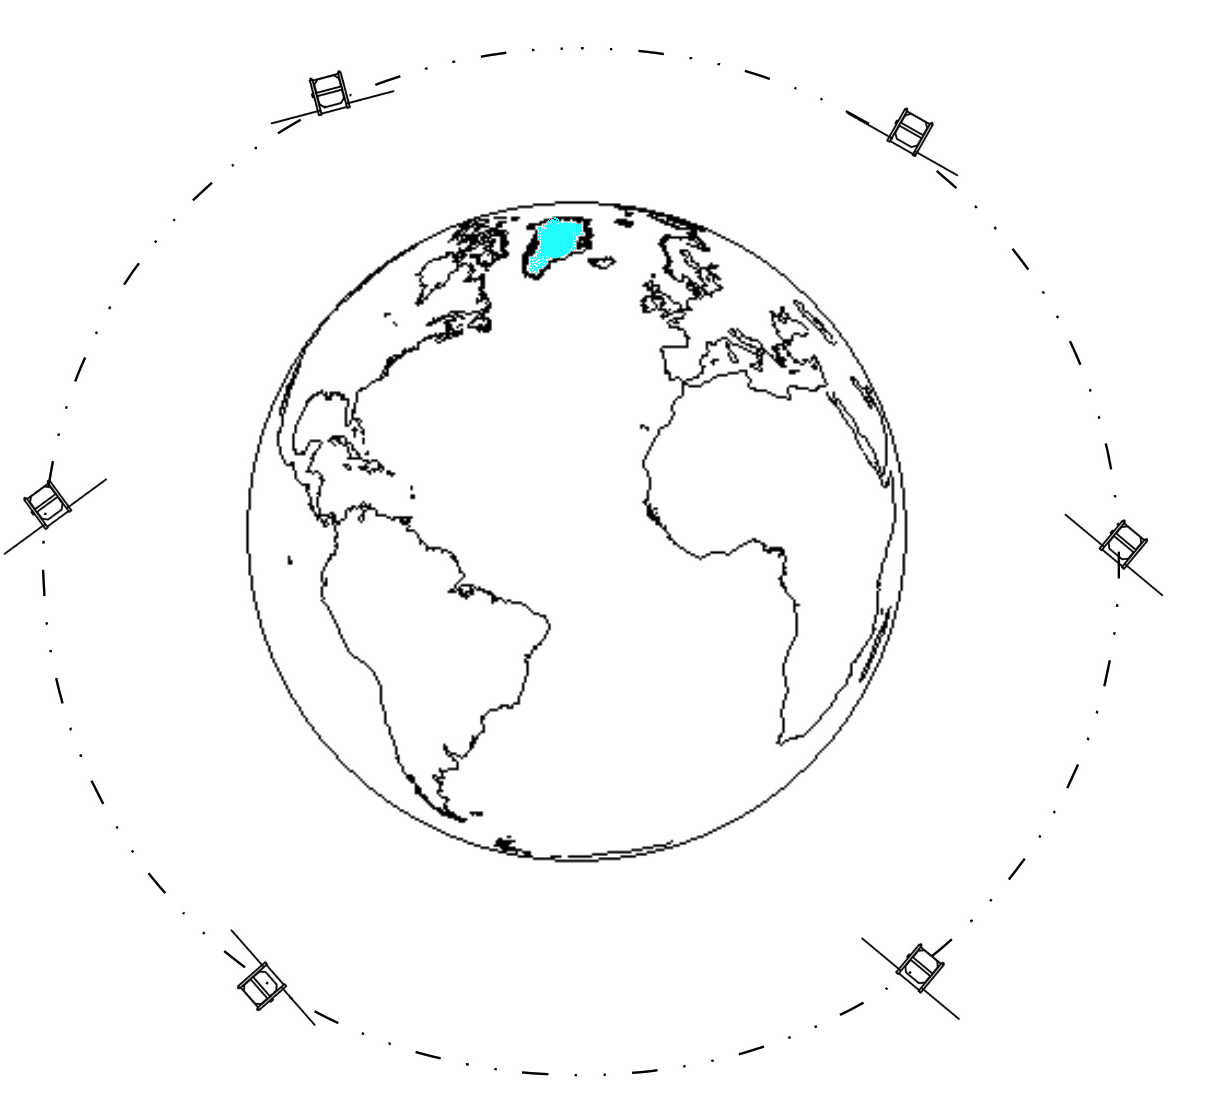
\includegraphics[width=0.6\linewidth]{figures/earth}
	\caption{Six satellites in flying formation on orbit}
	\label{fig:1}
\end{figure}
%
\section{About AAU-CubeSat}
The AAU-CubeSat shown in \figref{fig:pico} is a pico-satellite developed by Stanford University, but assembled at Aalborg University by students and used mainly for Low Earth Orbit (LEO)  tests.
\begin{figure}[H]
	\centering
	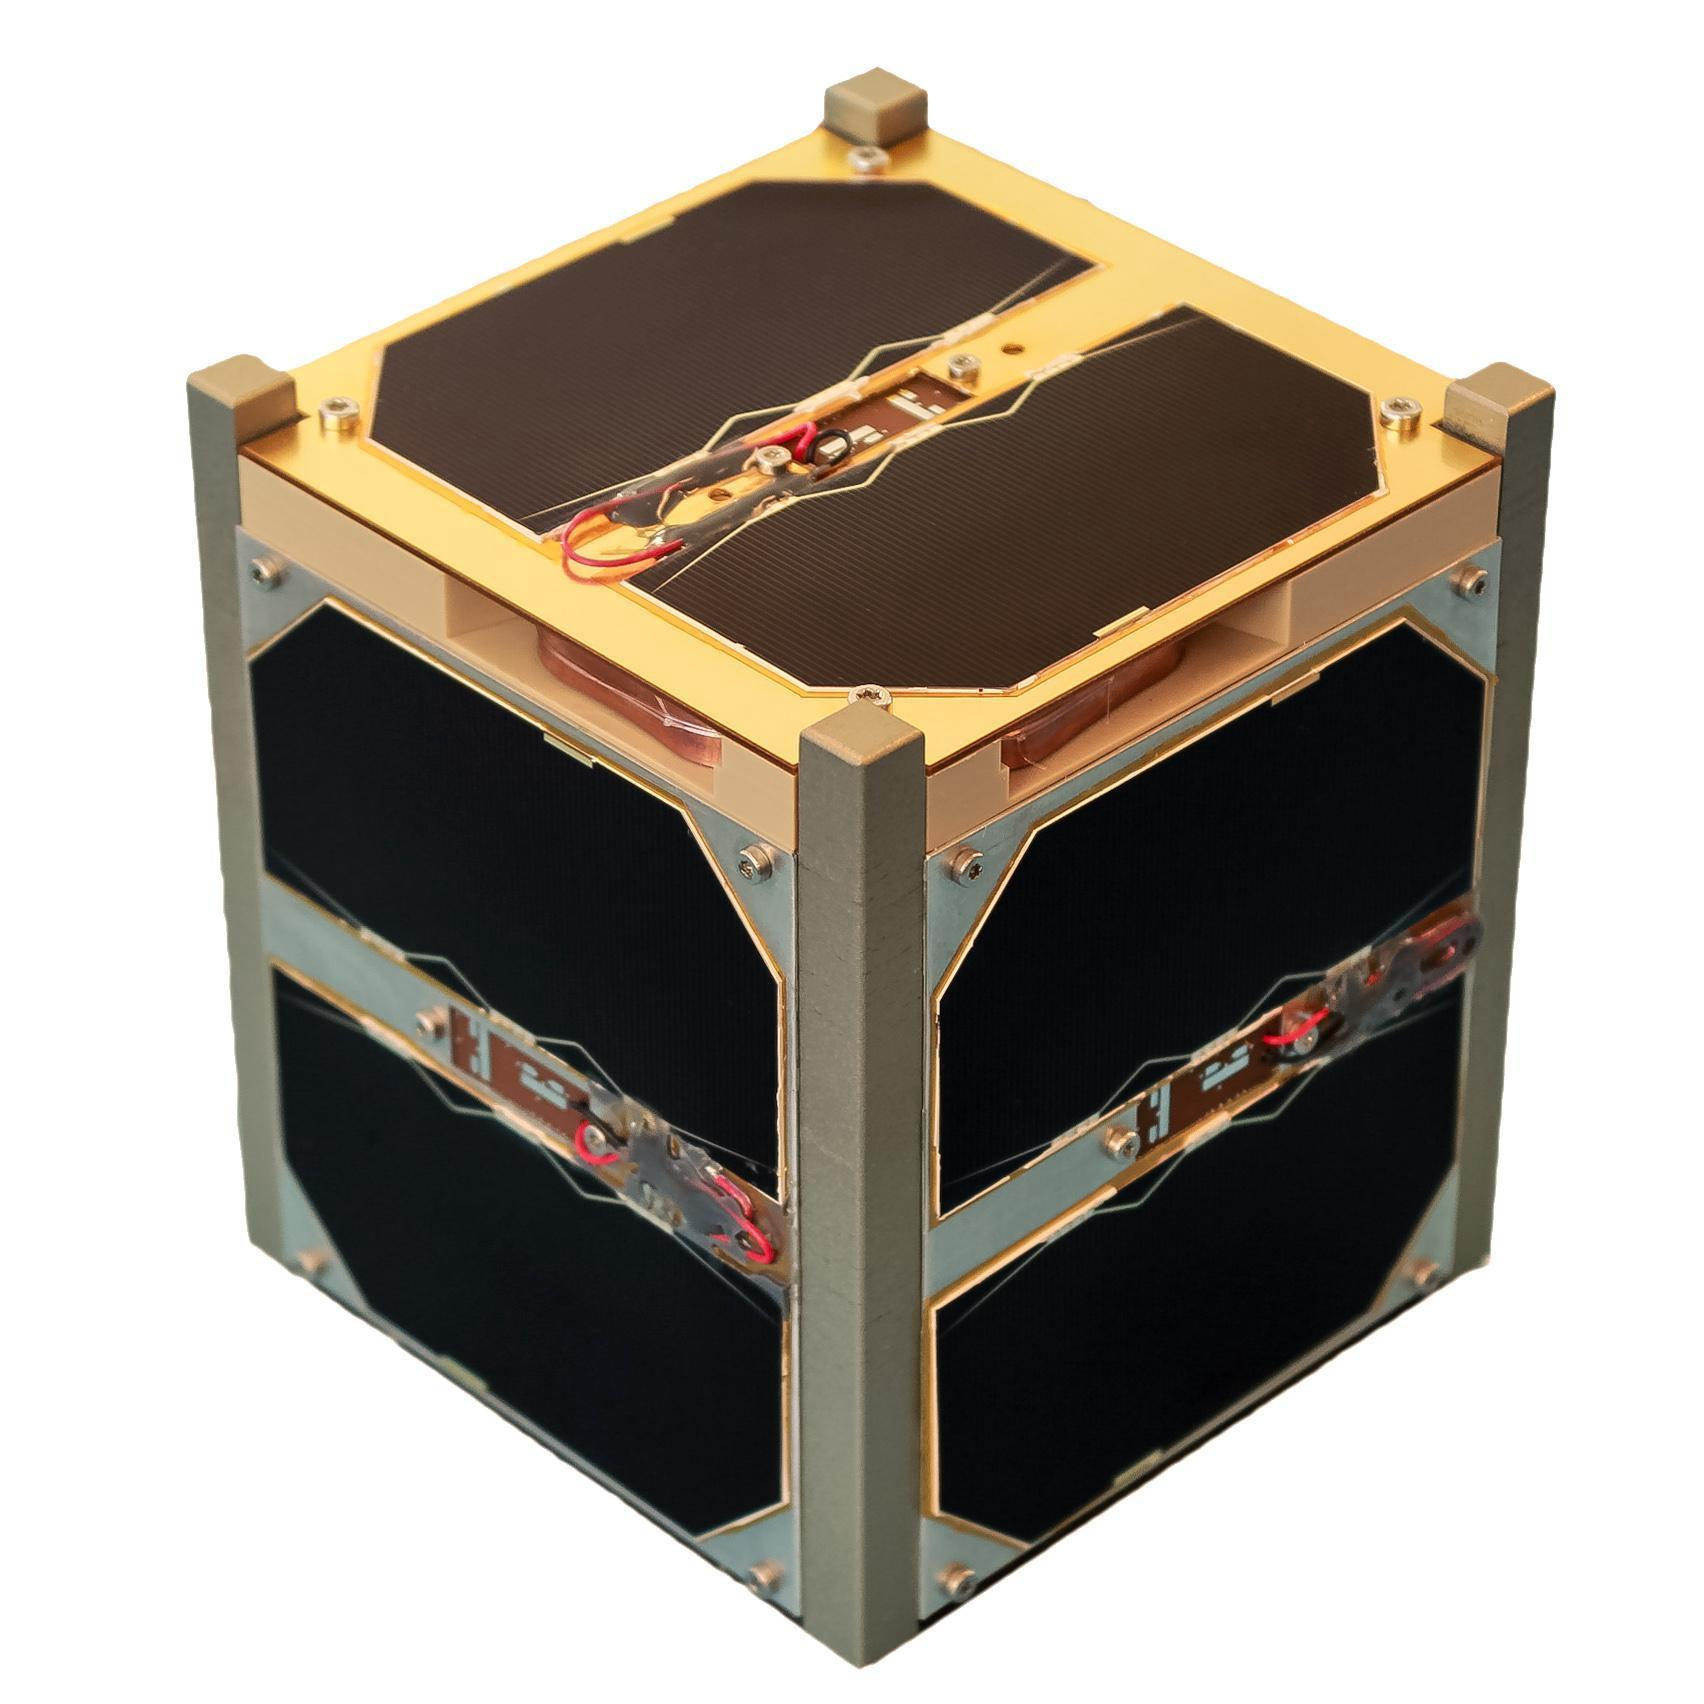
\includegraphics[width=0.3\linewidth]{figures/aau_cubsat}
	\caption{View of CubeSat satellite}
	\label{fig:pico}
\end{figure}
The pico-satellite is designed for LEO, therefore a few constraints are imposed. The CubeSat is limited in size and weight. The dimensions of the satellite are $10cm\times10cm\times30cm$, while the weight is around 1 kg. \fxnote{ref}

In order place the CubeSat on the orbit, a deployment system is used, called P-POD \fxnote{ref} This system uses the force of a spring to launch the satellite into space. The satellite will be placed inside the launch rocket as payload. By using this system, an important advantage is reducing the cost of the launch.
%
\section{AAU-CubeSat actuators}
The selection of attitude control components is important in order to meet the performance requirements. For this project, three magnetorquers and three momentum wheels have been chosen as actuators. Initially, using only three momentum wheels has been considered, but the downside of using only momentum wheels is that some amount of momentum can be stored in the wheel, which will imply having a way to take back all that momentum and use it. Therefore, there are multiple ways to release that torque, and one is to use magnetorquers. 

\textbf{Magnetorquers} are wire coils which generate an electromagnetic field. The field interacts with the Earth magnetic field and a torque is generated for stabilizing the satellite. An important aspect of the magnetorquer is when the momentum wheel reaches a maximum speed and can no longer produce the torque (this is referred as wheel saturation'), so a magnetorquer is used to extract the momentum from the wheel.
\begin{table}[H]
	\begin{minipage}[b]{0.49\linewidth}
		\centering
		\begin{figure}[H]
			\centering
			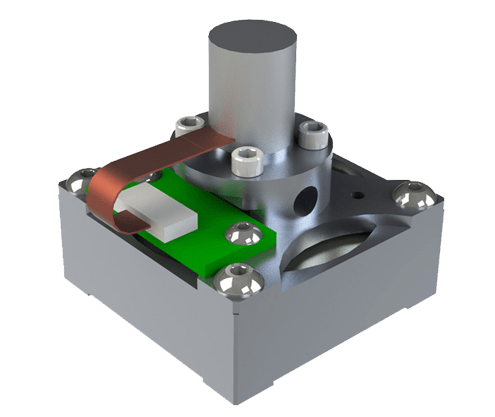
\includegraphics[width=0.5\linewidth]{figures/MW}
			\caption{Example of a momentum wheel for CubeSat}
			\label{fig:MW}
		\end{figure}
	\end{minipage}\hfill
	\begin{minipage}[b]{0.49\linewidth}
		\centering
		\begin{figure}[H]
			\centering
			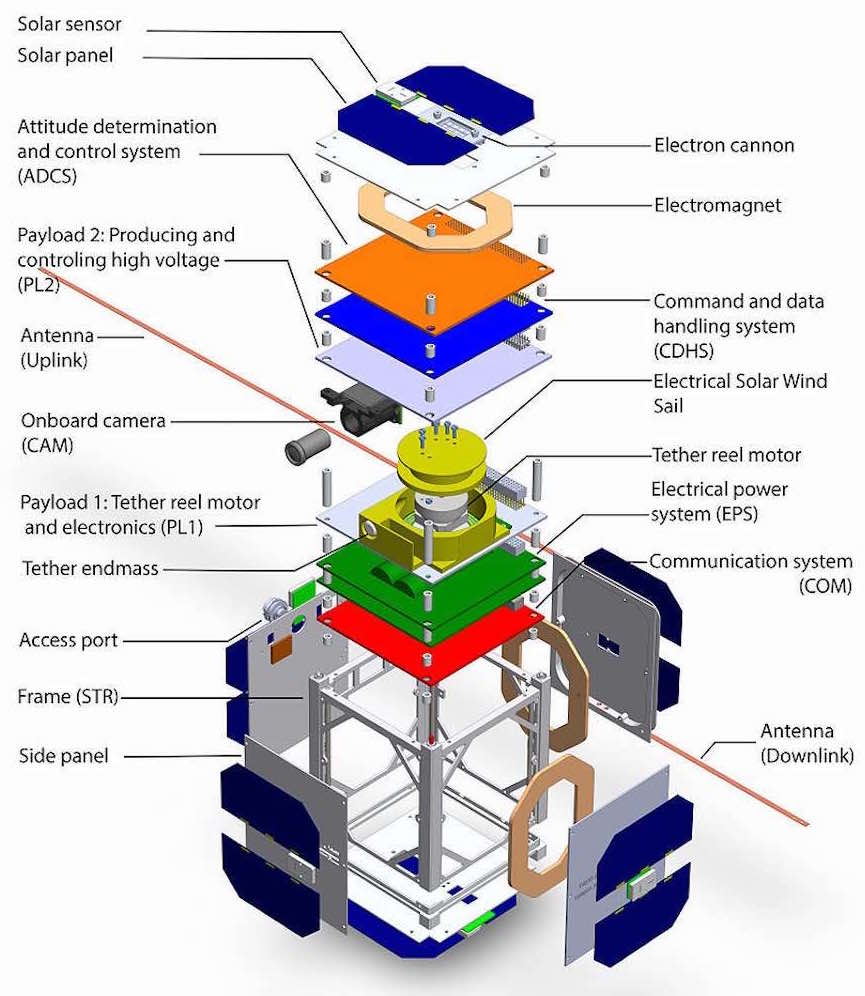
\includegraphics[width=1\linewidth]{figures/cubsat}
			\caption{Expanded view for CubeSat}
			\label{fig:cub}
		\end{figure}
	\end{minipage}
\end{table}
\textbf{Momentum wheels} shown in \figref{fig:MW} strength is that no information is needed about the magnetic field in order to control the CubeSat torque. These wheels are capable to store the momentum needed for maneuvering or pointing.

\textbf{Thrusters} ...description... Removing energy from the system it can be proved easily by using the drag force, but gaining energy it might be possible only if thrusters are used.
%  colloid thruster or "electrospray thruster"
%
\section{AAU-CubeSat sensors}
The CubeSat can sustain itself using solar pannels [ref in fig 2.4] with in the middle a sun sensor, which provide a vector equal to the direction of the sun and also a magnetometer that gives a vector of the Earth's magnetic field. Whether the Earth’s magnetic field is measured, or the sun vector, the objective is to use these sensors to deliver vector solutions for determining the satellite’s pointing and rotation rates.

\textbf{Magnetometer} is a sensor used for attitude control, which measure the direction and intensity of the magnetic field. The atittude is determined from the magnetometer by comparing the measure magnetic field with a referance field.

\textbf{Sun sensor} is used for delivering a vector of measurements from the Sun. (ref to the fig 2.4 )
%
\subsection{Pointing accuracy}
The required pointing accuracy when acquiring a photo is based on the a height from the picture is taken, in this case around 700 km above the Earth surface is going to cover approximately ?? km. 

\section{Coordinate frames}
In order to determine the attitude in three-dimensional space, various coordinate frames are defined.
\subsection{Reference Coordinate Systems}
In order to define an orbit around Earth, two specific Earth coordinate systems are defined. Both of them have their origin in the geometrical center of Earth and are named the Earth Centered Inertial (ECI) coordinate frame and the Earth Centered Earth Fixed (ECEF) coordinate frame. These can be seen in \figref{fig:ECI} and \figref{fig:ECEF}
\subsubsection{\textit{Earth Centered Inertial frame(ECI)}}
In order to describe the orbit formation of the satellite, the ECI frame shown in \figref{fig:ECI} is used, since it can be seen as a non-accelerating frame. The $z$ axis is pointing through the geographical north pole, the $x$ axis is crossing from the point where the equatorial of the earth and the vernal equinox met and the $y$ axis is the cross product of $x$ and $z$ creating a right-handed coordinate system. 
\begin{figure}[H]
	\centering
	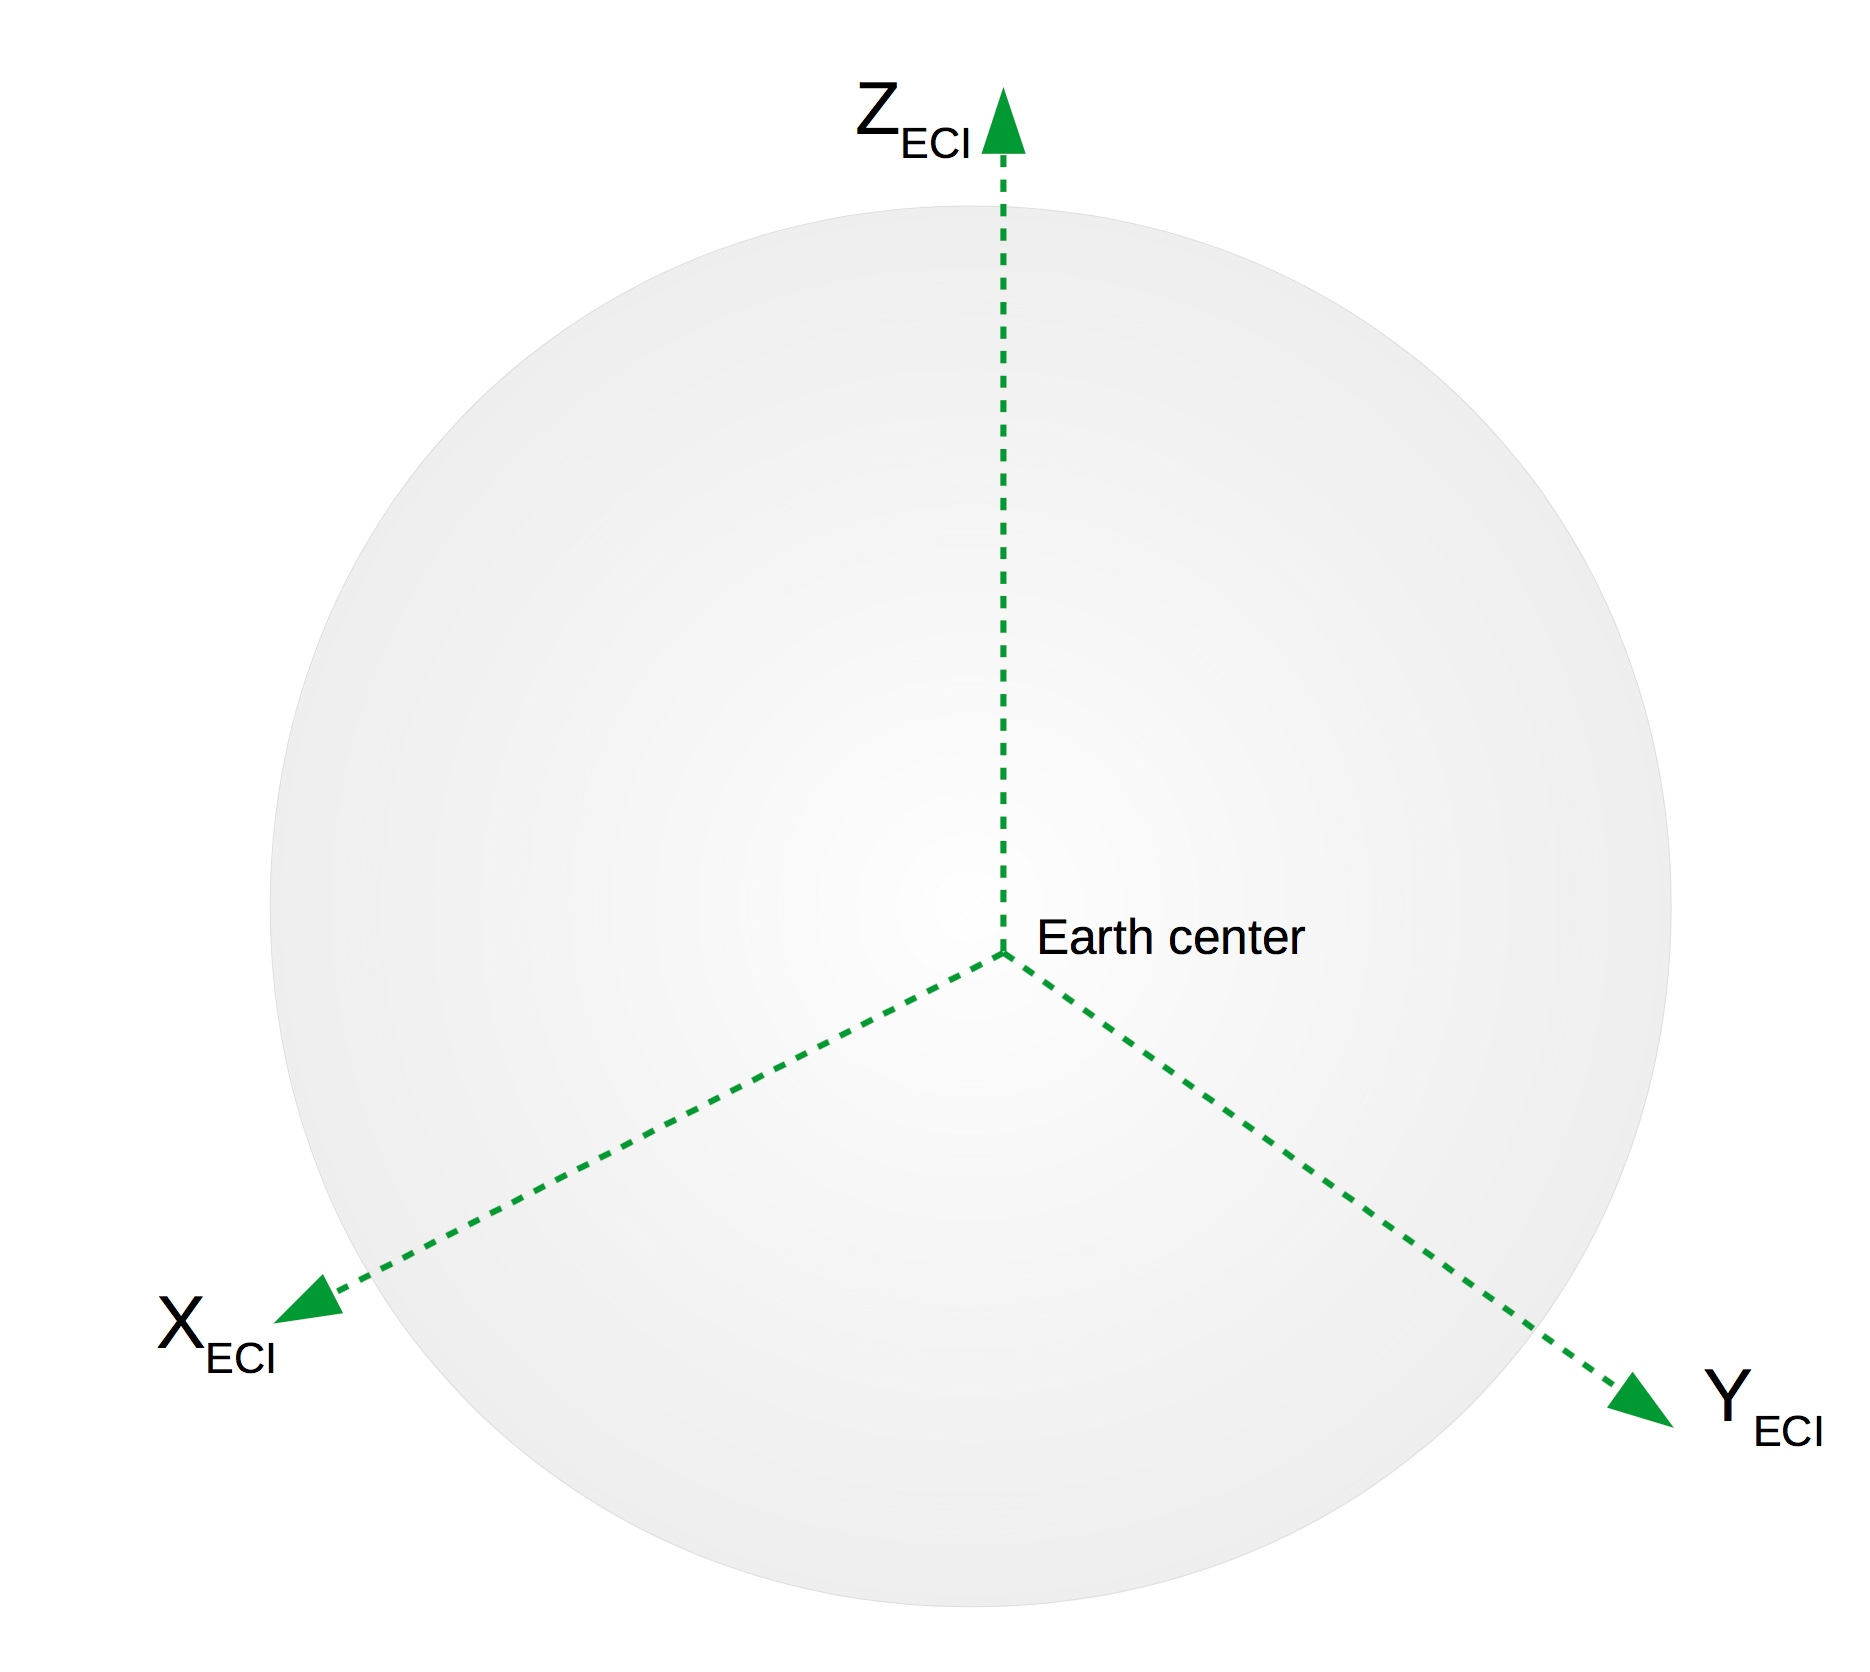
\includegraphics[width=0.5\linewidth]{figures/ECI}
	\caption{ECI coordinate frame}
	\label{fig:ECI}
\end{figure}
\subsubsection{\textit{Earth Centered Earth Fixed Frame (ECEF)}}
Another coordinate frame is the Earth Centered Earth Fixed (ECEF) coordinate frame shown in \figref{fig:ECEF}. In this case the X-axis is passing through the zero longitude, also known as Greenwich meredian, and the Z-axis parallel with the rotational axis. In this way the ECEF frame is fixed to the earth itself and rotates around with it.
\begin{figure}[H]
	\centering
	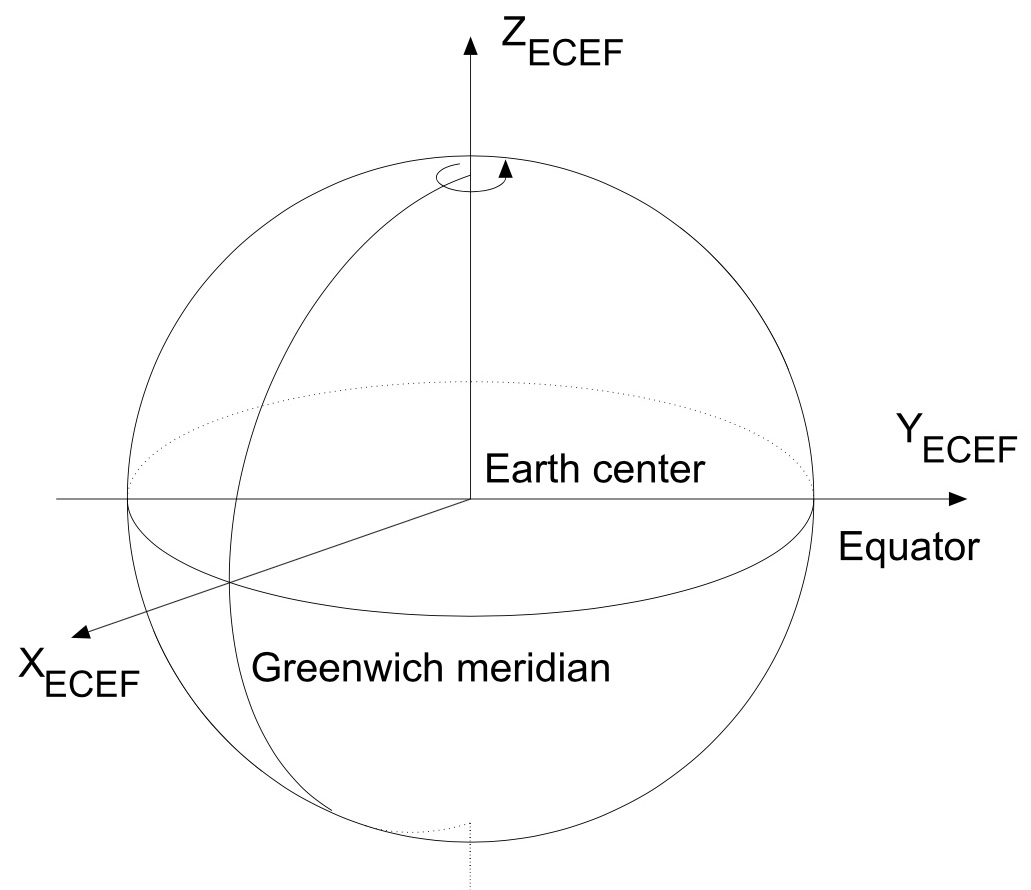
\includegraphics[width=0.5\linewidth]{figures/ECEF}
	\caption{ECEF coordinate frame}
	\label{fig:ECEF}
\end{figure}
\subsubsection{Satellite Coordinate Systems}
For the purpose of determining the attitude of the satellite, several coordinate systems are introduced. The attitude and position of the satellite is given as a rotation between the satellite fixed coordinate frames and the reference frames.
\subsubsection{\textit{Orbit Reference frame(ORF)}}
The orbit reference shown in \figref{fig:OFR} is a frame defined in Cartesian coordinates that can be seen as a non-changing frame with respect the earth and the satellite. The $z$ axis always pointing at the Nadir point and it is parallel to the $z_{e}$ axis o the inertial frame of the earth. The $x_{o}$ axis, it is parallel to the orbit plane and $y_{o}$ is the cross product of the $x_{o}$ and $z_{o}$. 
\begin{figure}[H]
	\centering
	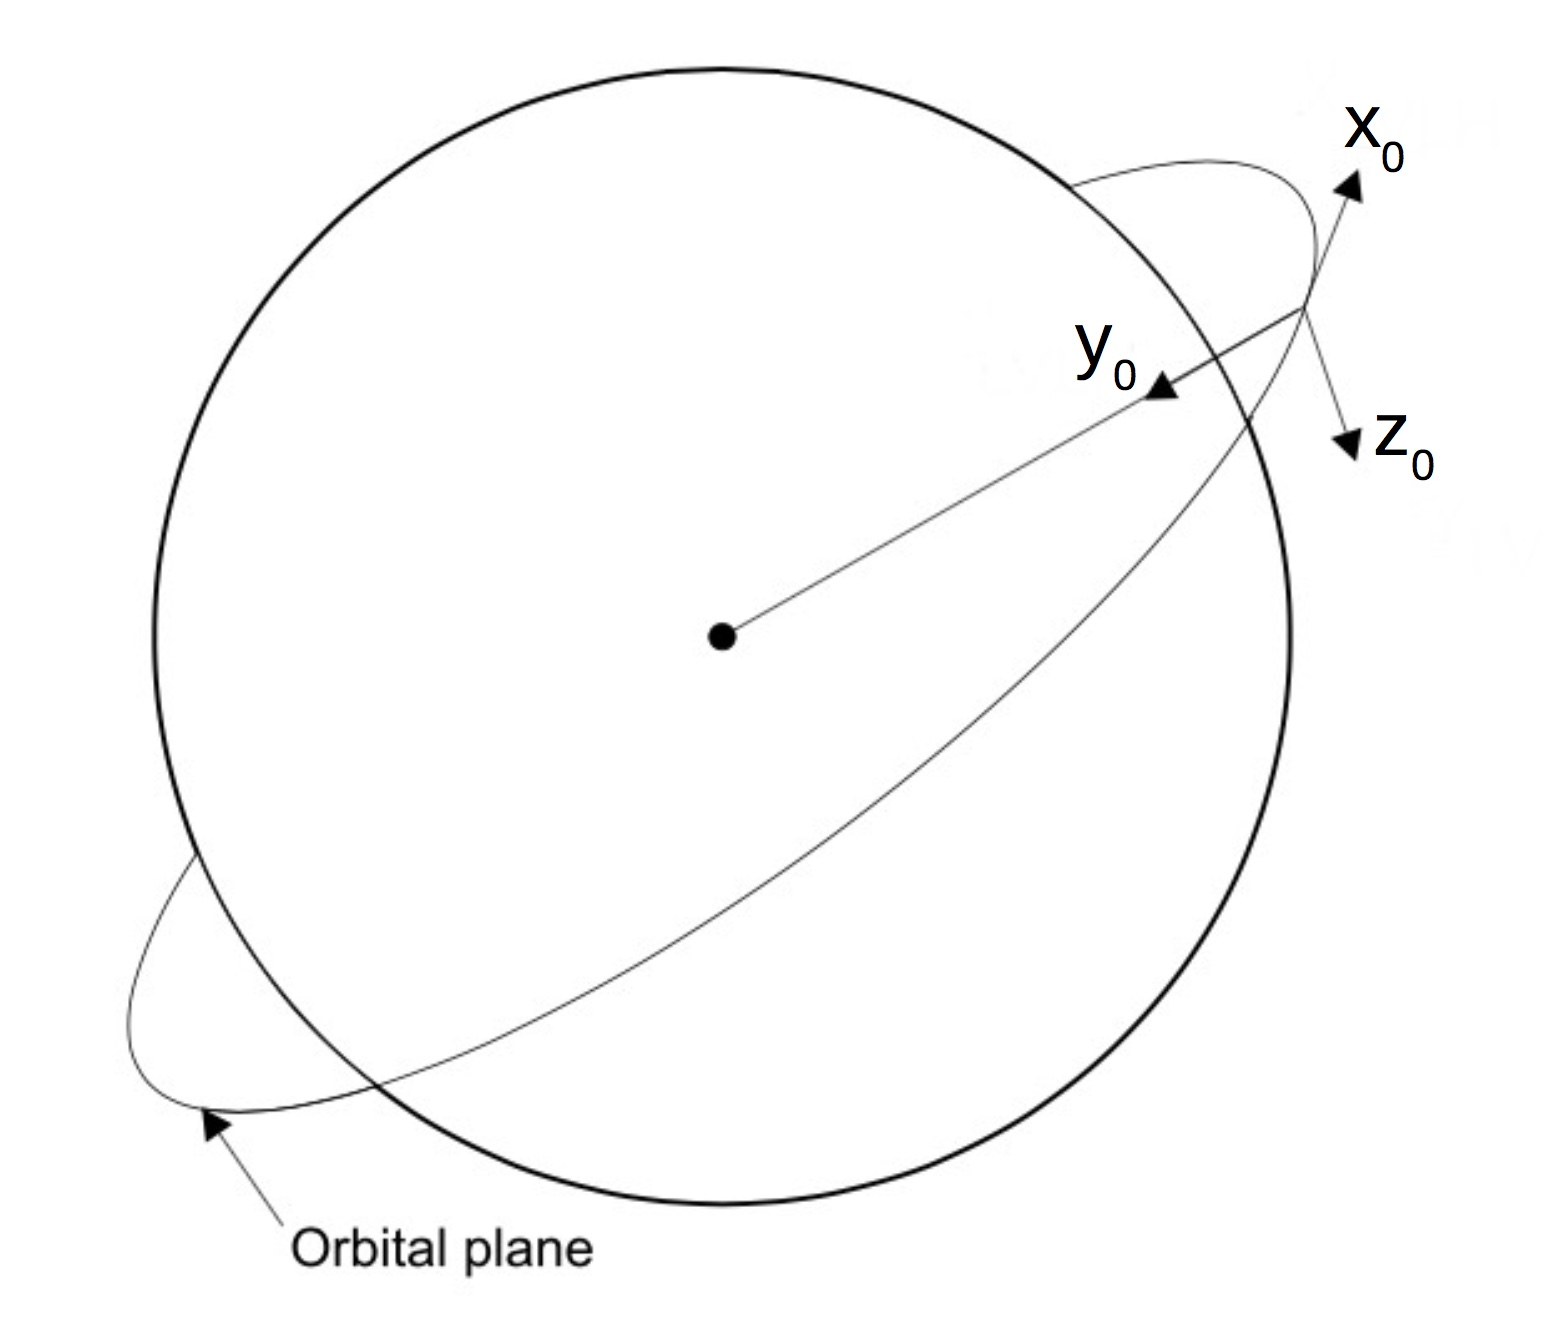
\includegraphics[width=0.4\linewidth]{figures/OFR}
	\caption{ORF coordinate frame}
	\label{fig:OFR}
\end{figure}
\subsubsection{\textit{Satellite Body Frame(SBF)}}
The satellite body frame is placed in the center of mass of the satellite as shown in  \figref{fig:frames}. 
\subsubsection{\textit{Satellite Controller frame(SCF)}}
In order to derive the kinematic equations, a controller reference frame seen in \figref{fig:frames} should be specified. It is located in the center of mass of the satellite and it is defined such that the axis of higher inertia $z_{c}$ pointing in the center of ECI and the $x_{c}$ axis with the smallest inertia, pointing along with  the orbit's $x_{o}$ 
\begin{figure}[H]
	\centering
	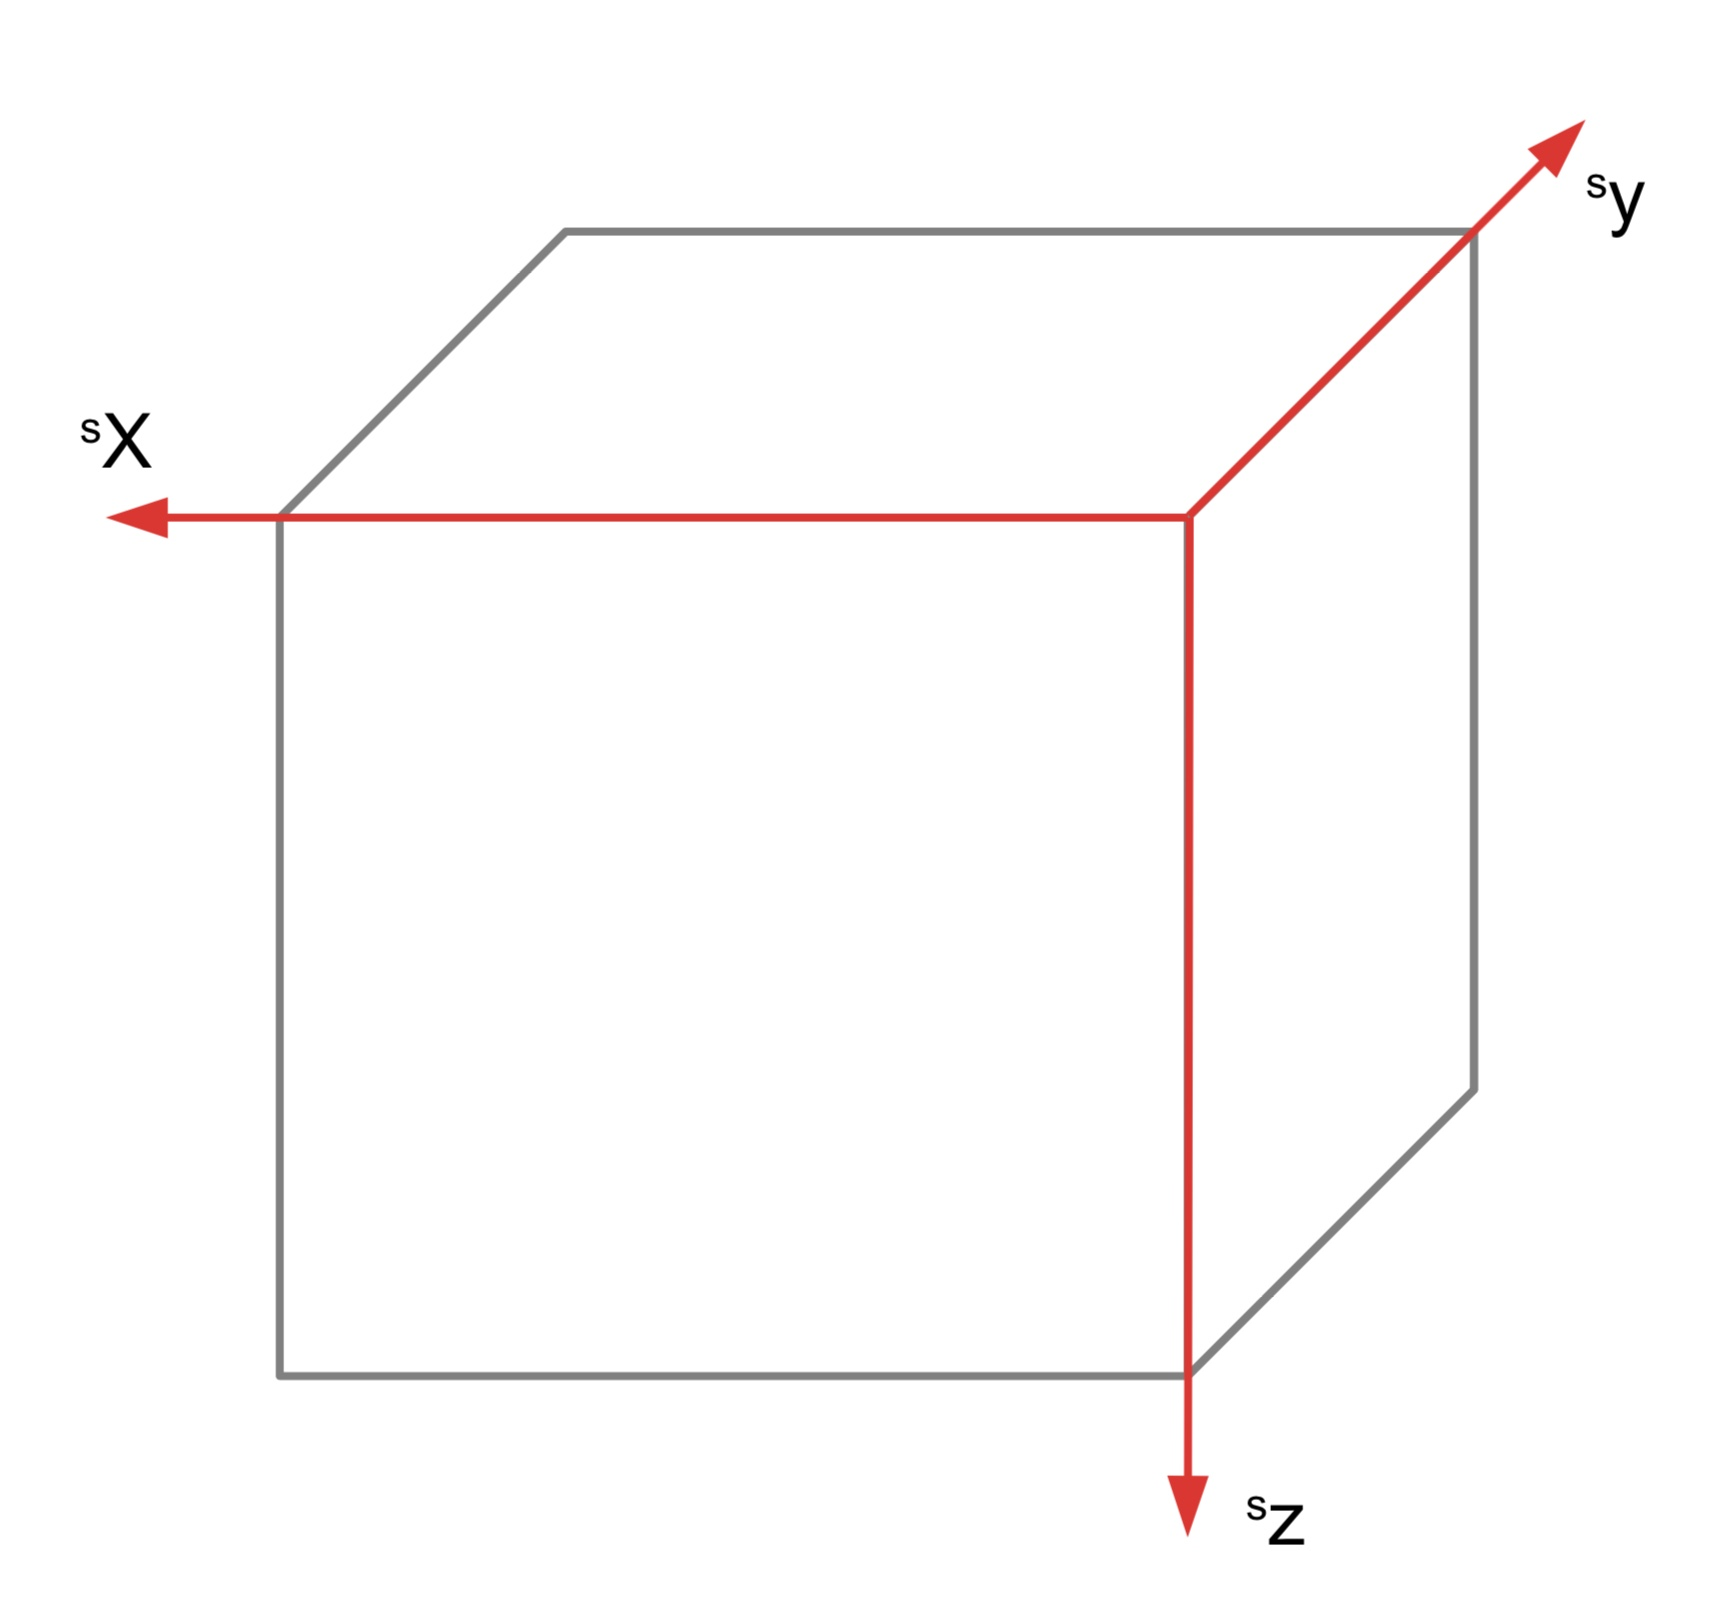
\includegraphics[width=0.4\linewidth]{figures/frames}
	\caption{Satellite body frame and satellite controller frame}
	\label{fig:frames}
\end{figure}

